%%=============================================================================
%% Conclusie
%%=============================================================================

\chapter{Conclusie}%
\label{ch:conclusie}

% TODO: Trek een duidelijke conclusie, in de vorm van een antwoord op de
% onderzoeksvra(a)g(en). Wat was jouw bijdrage aan het onderzoeksdomein en
% hoe biedt dit meerwaarde aan het vakgebied/doelgroep?
% Reflecteer kritisch over het resultaat. In Engelse teksten wordt deze sectie
% ``Discussion'' genoemd. Had je deze uitkomst verwacht? Zijn er zaken die nog
% niet duidelijk zijn?
% Heeft het onderzoek geleid tot nieuwe vragen die uitnodigen tot verder
%onderzoek?

\section{Bevindingen}
\paragraph{Enkelvoudige requests}
\textbf{REST - geen compressie}\newline
Zoals in hoofdstuk~\ref{ch:methodologie} voorgesteld werden de performantie testen voor de enkelvoudige requests, voor de voorgestelde dataset,
vier maal uitgevoerd en werd daarvan het gemiddelde genomen. Het resultaat is terug te vinden in tabel~\ref{tab:RESTenkelvoudig}.
Elke lijn op deze tabel komt overeen met een uitgevoerde request. In de eerste kolom worden het aantal items die werden opgevraagd weergegeven,
in de tweede kolom de grootte van de dataset, in MB, wanneer ze in JSON formaat naar een file worden weggeschreven,
daarna het tijdsverloop tussen de start van de request en het verkrijgen van de opgevraagde data in millie seconden. De laatste kolom geeft de de grootte van de
verzonden dataset, in MB, per seconde dat de request geduurd heeft.
Op figuur~\ref{fig:RESTenkelvoudig} wordt de snelheid, in MB/sec, weergegeven ten opzichte van de grootte van de verzonden dataset voor de vier sets van
calls die uitgevoerd werden, tevens werden trendlijnen voorzien volgens voortschrijdend gemiddelde over 3 metingen.\\

\begin{table}
    \centering
    \begin{tabular}{llll}
        \toprule
        \textbf{REST} & {Gemiddelde over 4 sets} & & \\
        \midrule
        Items / call & Grootte set (MB) & tijdsverloop (millies) & snelheid (Mb/s) \\
        1024 & 0,08 & 84,75 & 0,944 \\
        2048 & 0,17 & 136,25 & 1,248 \\
        4096 & 0,34 & 225,75 & 1,506 \\
        8192 & 0,68 & 438,5 & 1,551 \\
        9216 & 0,76 & 501,5 & 1,515 \\
        10240 & 0,85 & 546,25 & 1,556 \\
        11264 & 0,93 & 602,75 & 1,543 \\
        12288 & 1,02 & 644,5 & 1,583 \\
        13312 & 1,1 & 690,75 & 1,592 \\
        14336 & 1,19 & 742,25 & 1,603 \\
        15360 & 1,27 & 807,25 & 1,573 \\
        16384 & 1,36 & 857,5 & 1,586 \\
        20480 & 1,7 & 1057 & 1,608 \\
        24576 & 2,04 & 1277,5 & 1,597 \\
        28672 & 2,38 & 1468,75 & 1,620 \\
        32768 & 2,72 & 1676,5 & 1,622 \\
        36864 & 3,06 & 1894 & 1,616 \\
        40960 & 3,4 & 2104,5 & 1,616 \\
        45056 & 3,74 & 2309,75 & 1,619 \\
        49152 & 4,07 & 2546,5 & 1,598 \\
        53248 & 4,41 & 2753,5 & 1,602 \\
        57344 & 4,75 & 3208,5 & 1,480 \\
        61440 & 5,09 & 3165,5 & 1,608 \\
        65536 & 5,43 & 3347,5 & 1,622 \\
        131072 & 10,87 & 6759,5 & 1,608 \\
        262144 & 21,73 & 13689,75 & 1,587 \\
        524288 & 43,46 & 27022,25 & 1,608 \\
         &  &  &  \\
        gemiddelde: &  &  & 1,549 \\
        max: &  &  & 1,622 \\
        min: &  &  & 0,944 \\
        \bottomrule
    \end{tabular}
    \caption{REST - enkelvoudige requests: snelheid vs. datasets van vari\"erende grootte (gemiddelde over 4 sets)}
    \label{tab:RESTenkelvoudig}
\end{table}

\begin{figure}[ht]
    \centering
    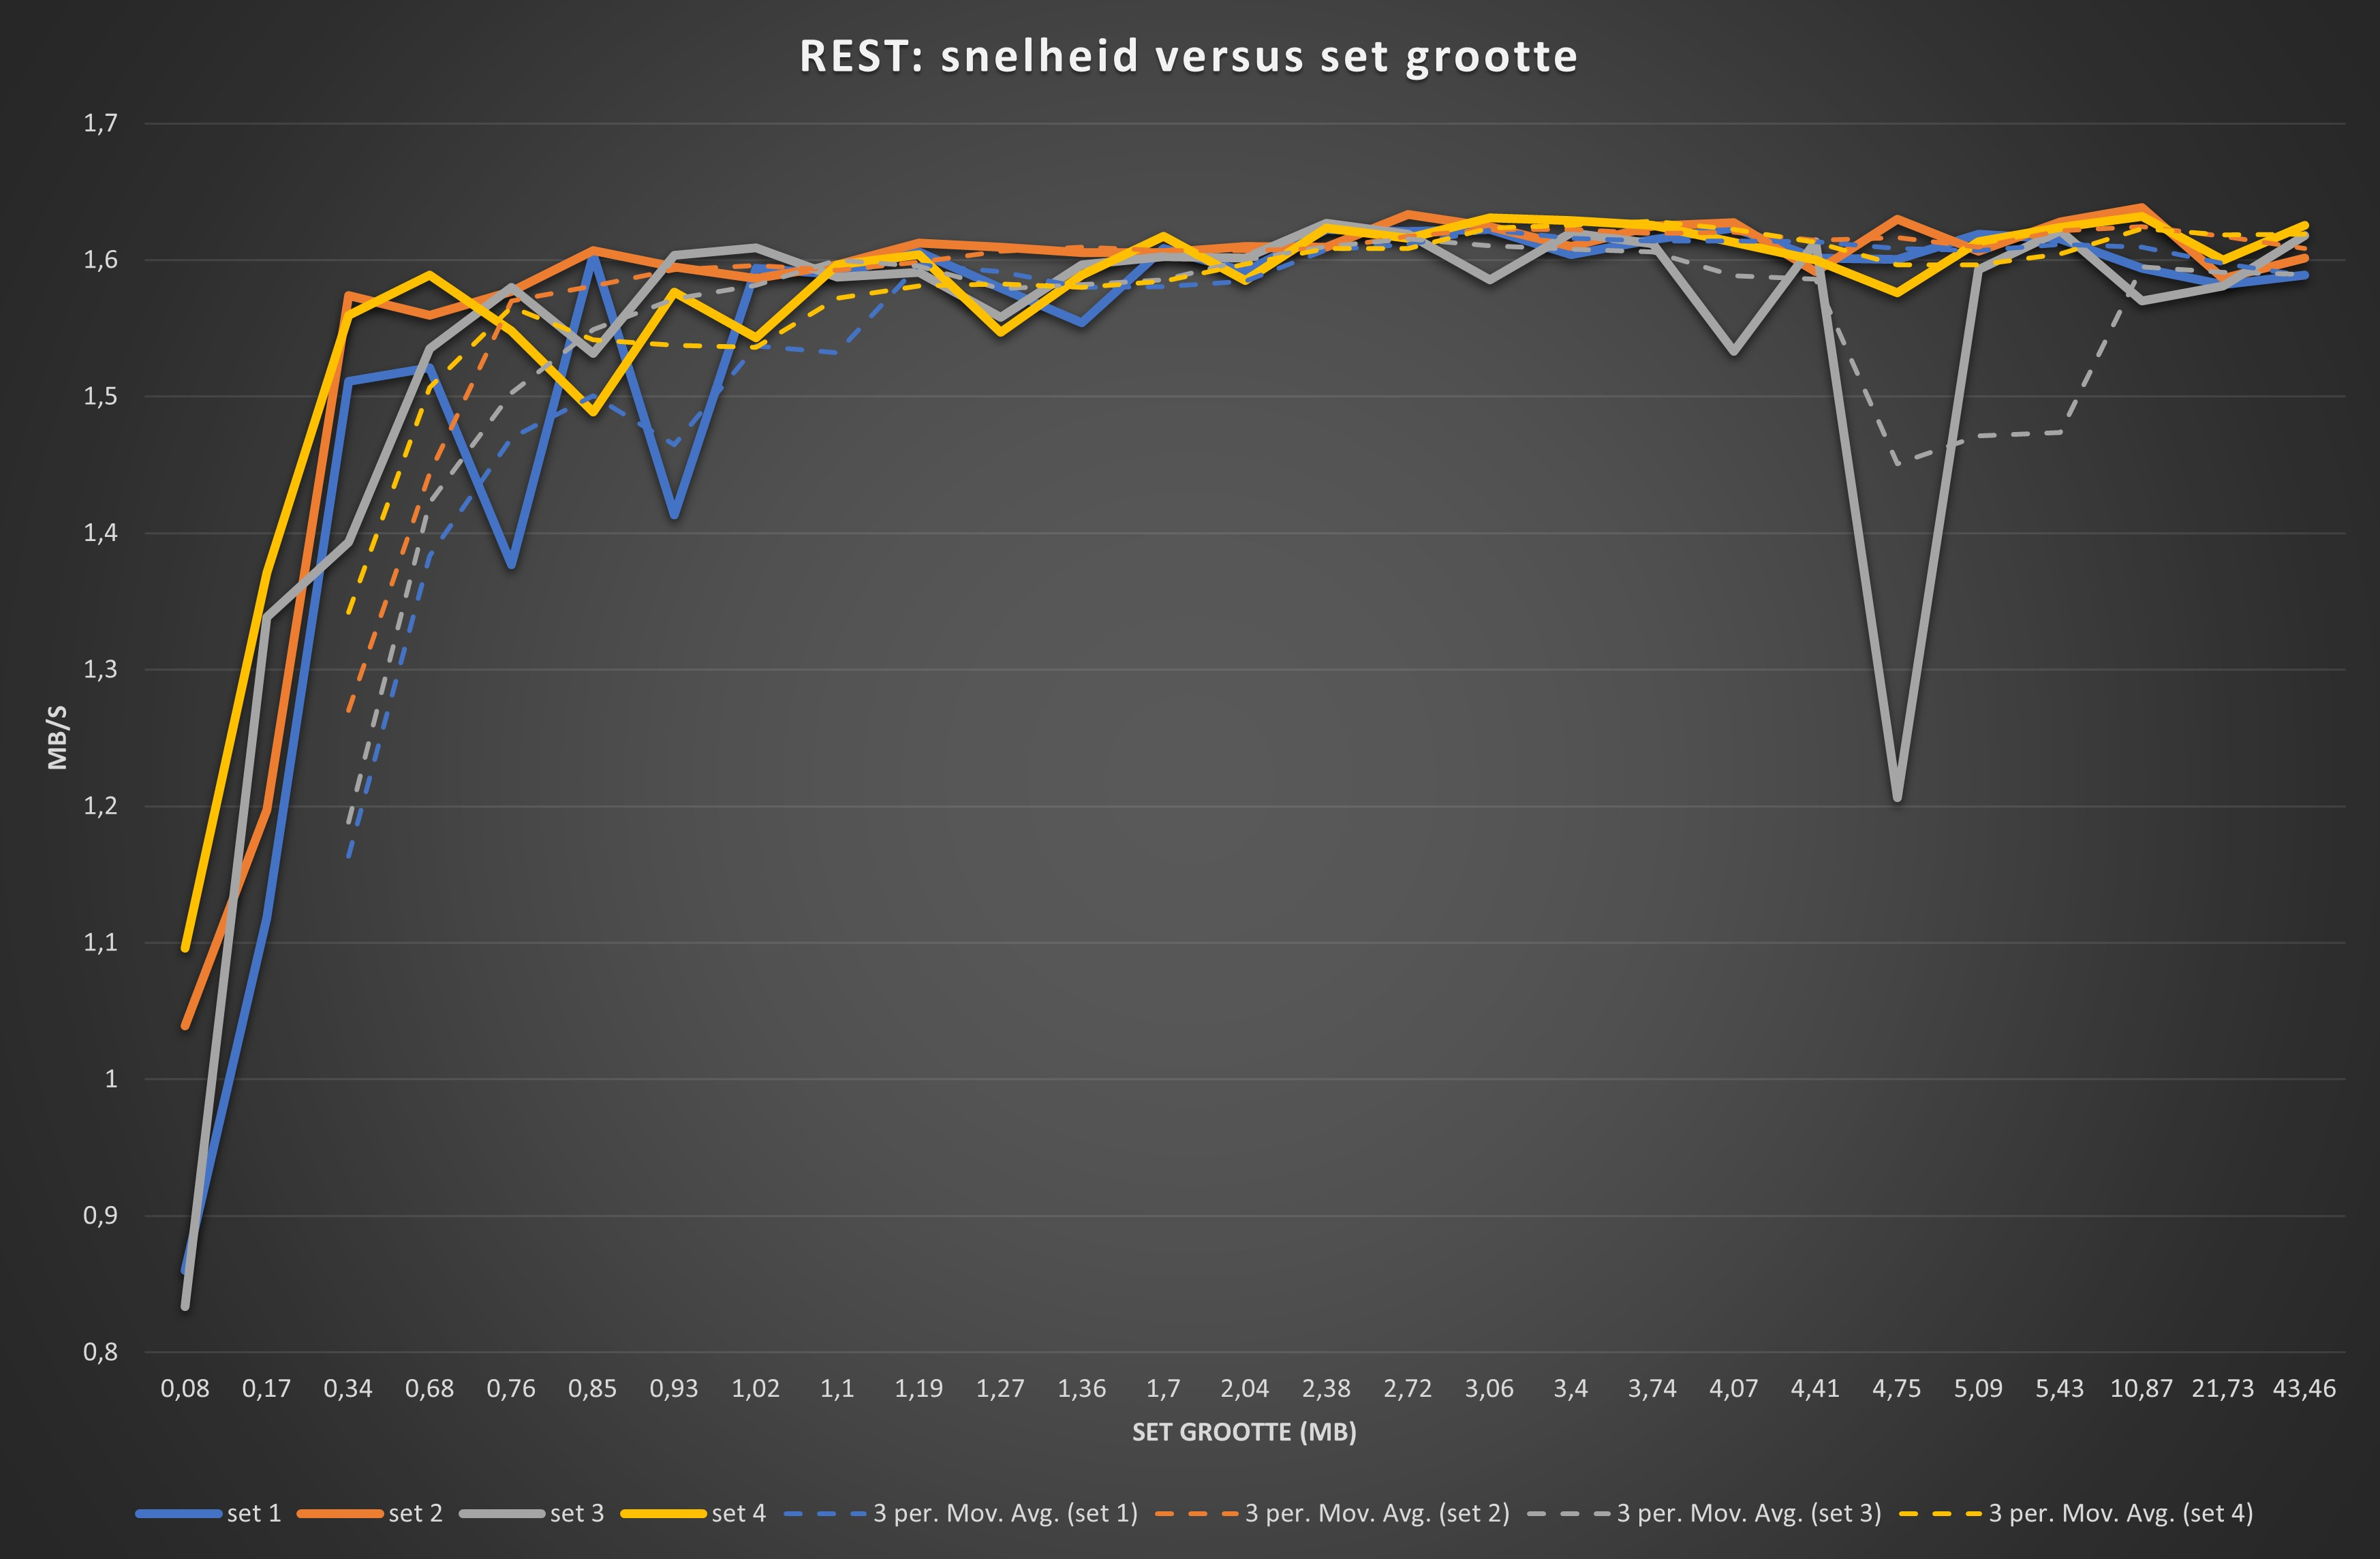
\includegraphics[width=1.0\linewidth]{REST_singular}
    \caption{REST - enkelvoudige requests: snelheid vs. datasets van vari\"erende grootte}
    \label{fig:RESTenkelvoudig}
\end{figure}

\textbf{REST - met compressie}\newline
Het gemiddelde van de performantiemeting van de enkelvoudige requests met het REST API waarbij de data door de server gecomprimeerd werd alvorens te verzenden
en bij de client weer gedecomprimeerd is terug te vinden in tabel~\ref{tab:RESTcompressieenkelvoudig}
Op figuur~\ref{fig:RESTcompressieenkelvoudig} wordt de snelheid, in MB/sec, weergegeven ten opzichte van de grootte van de verzonden dataset voor de vier sets van
calls die uitgevoerd werden, tevens werden trendlijnen voorzien volgens voortschrijdend gemiddelde over 3 metingen.\\

\begin{table}
    \centering
    \begin{tabular}{llll}
        \toprule
        \textbf{REST gecomprimeerd} & {Gemiddelde over 4 sets} &  & \\
        \midrule
        Items / call & Grootte set (MB) & tijdsverloop (millies) & snelheid (MB/s) \\
        1024 & 0,08 & 84,75 & 0,944 \\
        2048 & 0,17 & 85,25 & 1,994 \\
        4096 & 0,34 & 99,5 & 3,417 \\
        8192 & 0,68 & 151,5 & 4,488 \\
        9216 & 0,76 & 201 & 3,781 \\
        10240 & 0,85 & 208,25 & 4,082 \\
        11264 & 0,93 & 216,25 & 4,301 \\
        12288 & 1,02 & 230 & 4,435 \\
        13312 & 1,1 & 214 & 5,140 \\
        14336 & 1,19 & 245 & 4,857 \\
        15360 & 1,27 & 240,5 & 5,281 \\
        16384 & 1,36 & 255,25 & 5,328 \\
        20480 & 1,7 & 316 & 5,380 \\
        24576 & 2,04 & 371,75 & 5,488 \\
        28672 & 2,38 & 442,5 & 5,379 \\
        32768 & 2,72 & 488,25 & 5,571 \\
        36864 & 3,06 & 554 & 5,523 \\
        40960 & 3,4 & 593,25 & 5,731 \\
        45056 & 3,74 & 665,25 & 5,622 \\
        49152 & 4,07 & 734,25 & 5,543 \\
        53248 & 4,41 & 860,25 & 5,126 \\
        57344 & 4,75 & 960,25 & 4,947 \\
        61440 & 5,09 & 1003,5 & 5,072 \\
        65536 & 5,43 & 1164,25 & 4,664 \\
        131072 & 10,87 & 2079,75 & 5,227 \\
        262144 & 21,73 & 3909 & 5,559 \\
        524288 & 43,46 & 8374,25 & 5,190 \\
         &  &  &  \\
        gemiddelde: &  &  & 4,743 \\
        max: &  &  & 5,731 \\
        min: &  &  & 0,944 \\
        \bottomrule
    \end{tabular}
    \caption{REST gecomprimeerd  - enkelvoudige requests: snelheid vs. datasets van vari\"erende grootte (gemiddelde over 4 sets)}
    \label{tab:RESTcompressieenkelvoudig}
\end{table}


\begin{figure}[ht]
    \centering
    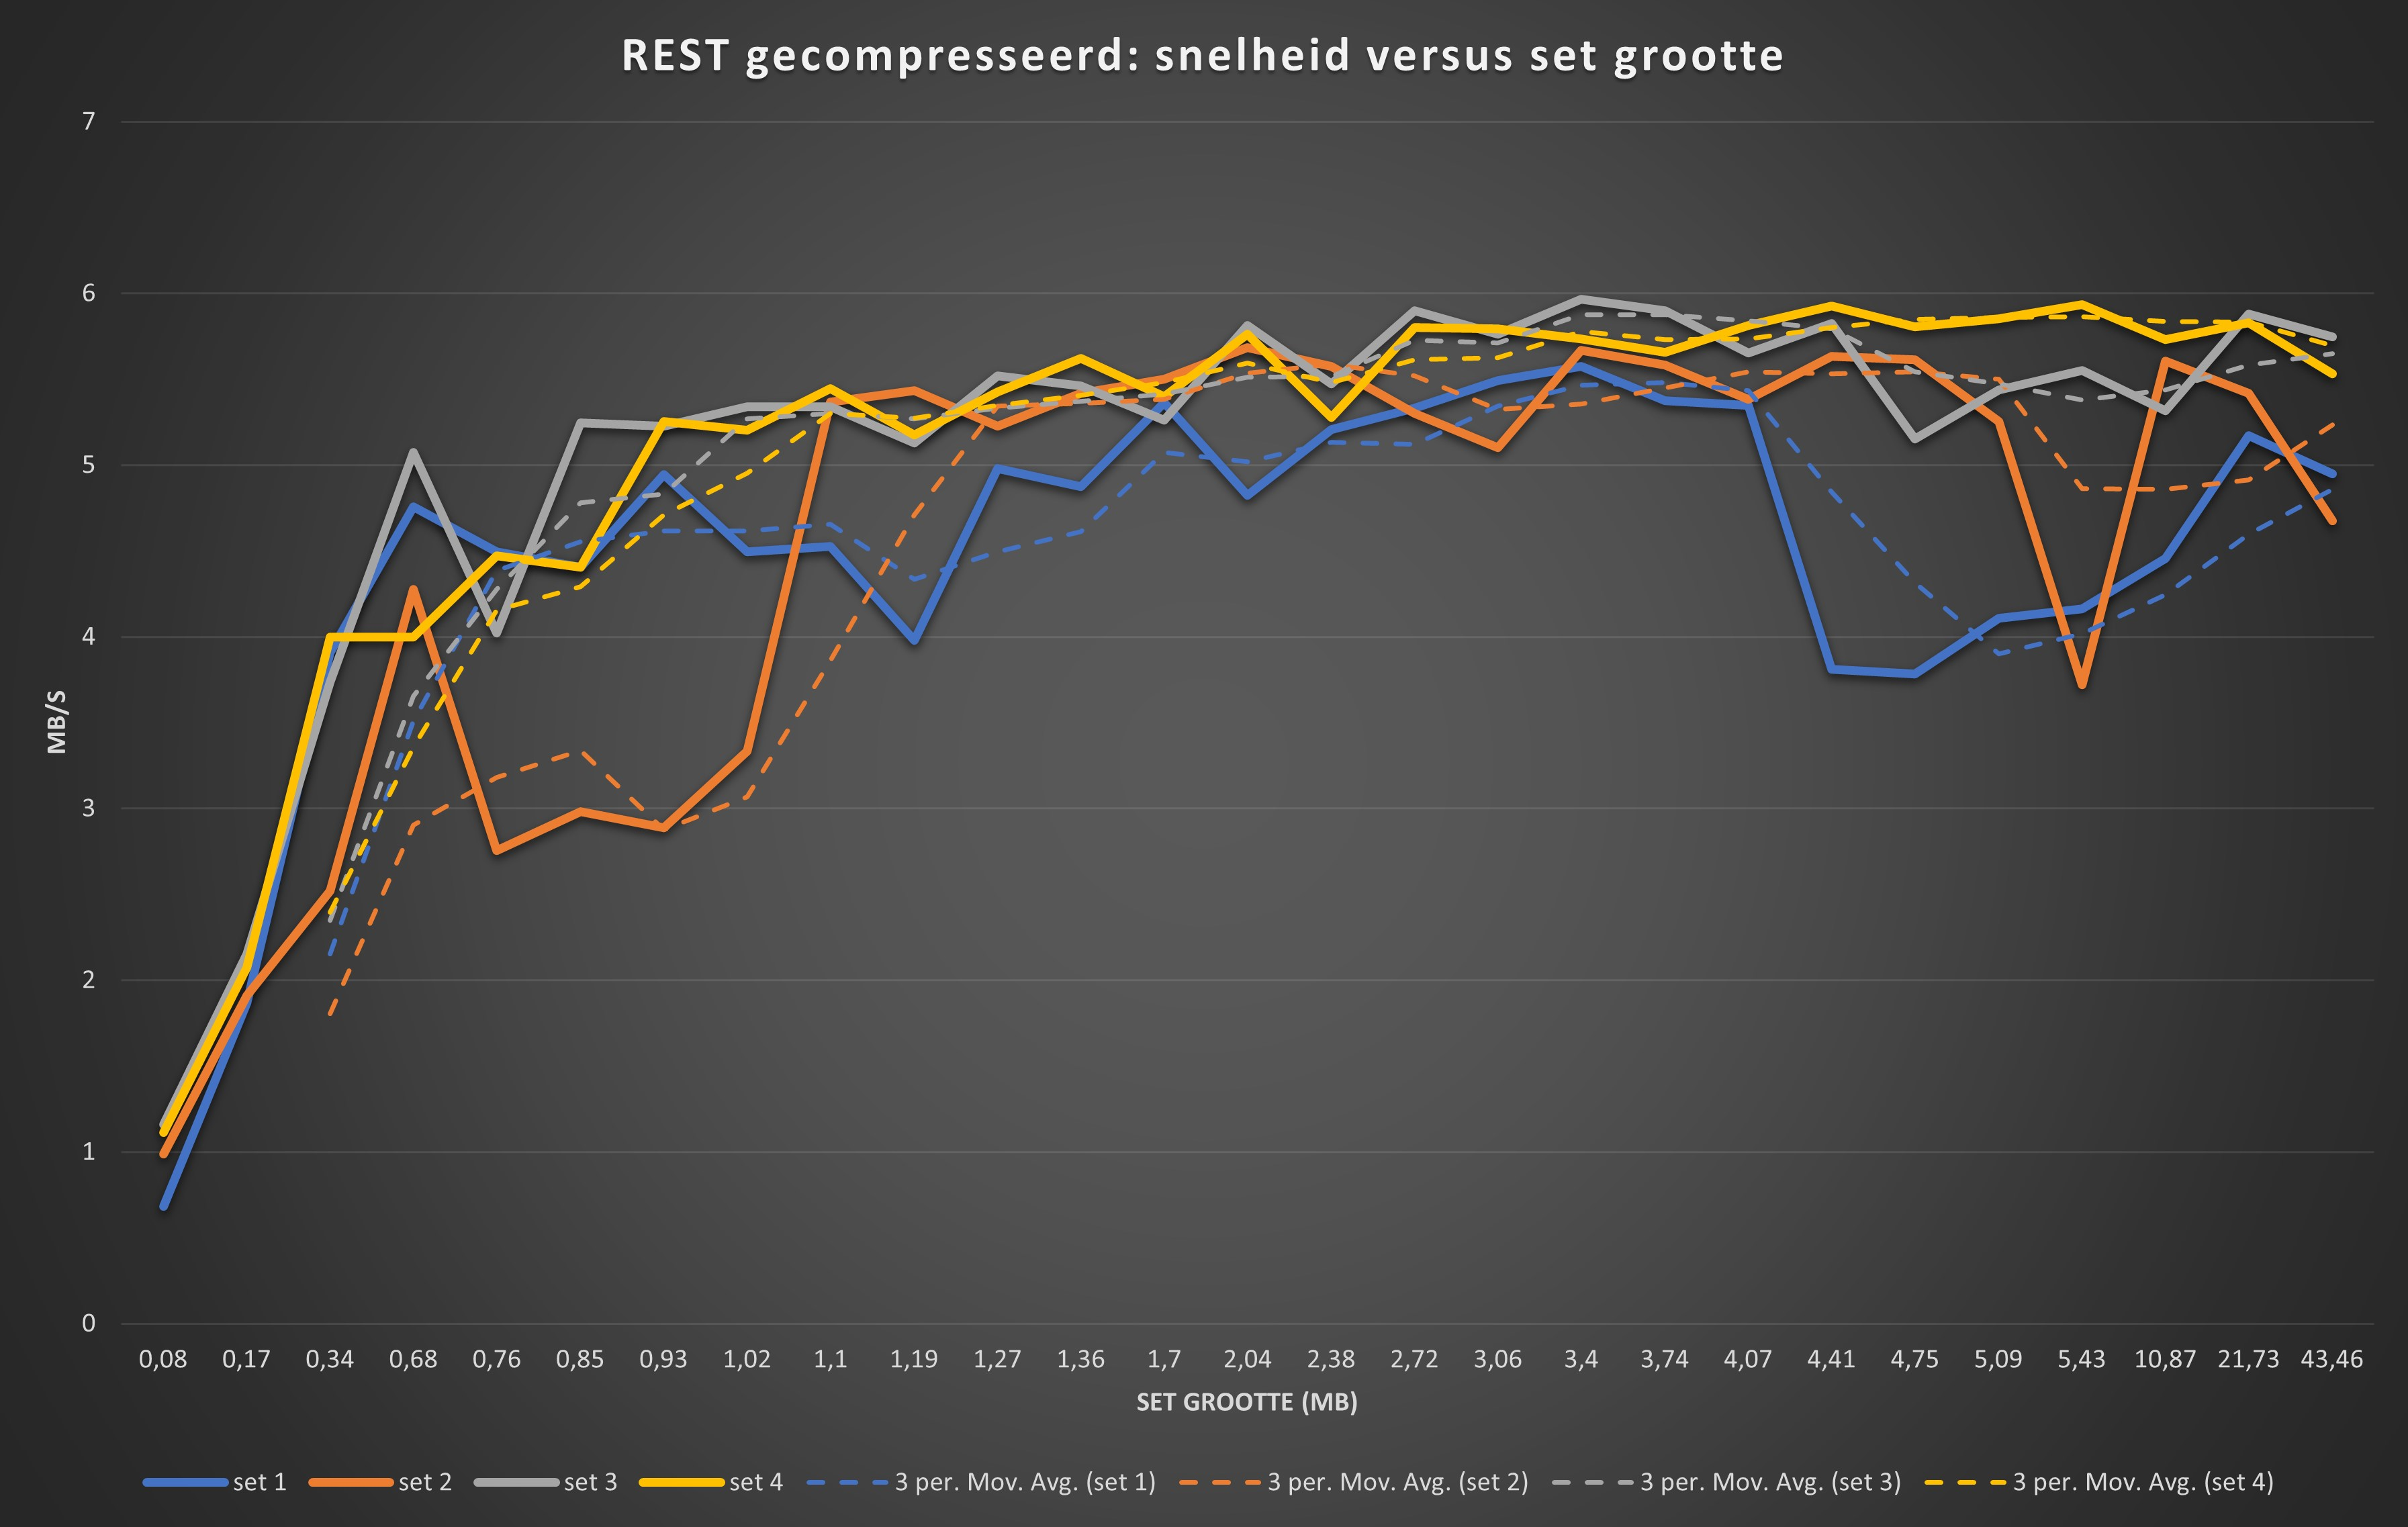
\includegraphics[width=1.0\linewidth]{REST_compressed_singular}
    \caption{REST gecomprimeerd - enkelvoudige requests: snelheid vs. datasets van vari\"erende grootte}
    \label{fig:RESTcompressieenkelvoudig}
\end{figure}

\textbf{gRPC - Uni}\newline
Het gemiddelde van de performantiemeting van de enkelvoudige requests met de gRPC API functie getPeople, welke een object van het type Uni teruggeeft, zijn
terug te vinden in tabel~\ref{tab:gRPCUnienkelvoudig}
Op figuur~\ref{fig:RESTcompressieenkelvoudig} wordt de snelheid in MB/sec weergegeven ten opzichte van de grootte van de verzonden dataset voor de vier sets van
calls die uitgevoerd werden, tevens werden trendlijnen voorzien volgens voortschrijdend gemiddelde over 3 metingen.\\
Op figuur~\ref{fig:gRPCUnienkelvoudig} wordt de snelheid, in MB/sec, weergegeven ten opzichte van de grootte van de verzonden dataset voor de vier sets van
calls die uitgevoerd werden, tevens werden trendlijnen voorzien volgens voortschrijdend gemiddelde over 3 metingen.\\

\begin{table}
    \centering
    \begin{tabular}{llll}
        \toprule
        \textbf{gRPC Uni} & {Gemiddelde over 4 sets} &  & \\
        \midrule
        Items / call & Groote subset (MB) & tijdsverloop (millies) & snelheid (MB/s) \\
        1024 & 0,08 & 47,25 & 1,693121693 \\
        2048 & 0,17 & 79,25 & 2,14511041 \\
        4096 & 0,34 & 85 & 4 \\
        8192 & 0,68 & 142,5 & 4,771929825 \\
        9216 & 0,76 & 159,5 & 4,764890282 \\
        10240 & 0,85 & 182,5 & 4,657534247 \\
        11264 & 0,93 & 187,5 & 4,96 \\
        12288 & 1,02 & 217 & 4,700460829 \\
        13312 & 1,1 & 219 & 5,02283105 \\
        14336 & 1,19 & 238,5 & 4,98951782 \\
        15360 & 1,27 & 265,25 & 4,78793591 \\
        16384 & 1,36 & 268 & 5,074626866 \\
        20480 & 1,7 & 339 & 5,014749263 \\
        24576 & 2,04 & 407,5 & 5,006134969 \\
        28672 & 2,38 & 463,75 & 5,132075472 \\
        32768 & 2,72 & 526 & 5,171102662 \\
        36864 & 3,06 & 582,25 & 5,255474453 \\
        40960 & 3,4 & 647,25 & 5,252993434 \\
        45056 & 3,74 & 718,75 & 5,203478261 \\
        49152 & 4,07 & 763,5 & 5,330713818 \\
        53248 & 4,41 & 828 & 5,326086957 \\
        57344 & 4,75 & 892,25 & 5,323620062 \\
        61440 & 5,09 & 966,75 & 5,265063357 \\
        65536 & 5,43 & 1021 & 5,318315377 \\
        131072 & 10,87 & 2007,75 & 5,41402067 \\
        262144 & 21,73 & 4044,25 & 5,373060518 \\
        524288 & 43,46 & 8136 & 5,341691249 \\
         &  &  &  \\
        gemiddelde: &  &  & 4,825797757 \\
        max: &  &  & 5,41402067 \\
        min: &  &  & 1,693121693 \\
        \bottomrule
    \end{tabular}
    \caption{gRPC Uni - enkelvoudige requests: snelheid vs. datasets van vari\"erende grootte (gemiddelde over 4 sets)}
    \label{tab:gRPCUnienkelvoudig}
\end{table}


\begin{figure}[ht]
    \centering
    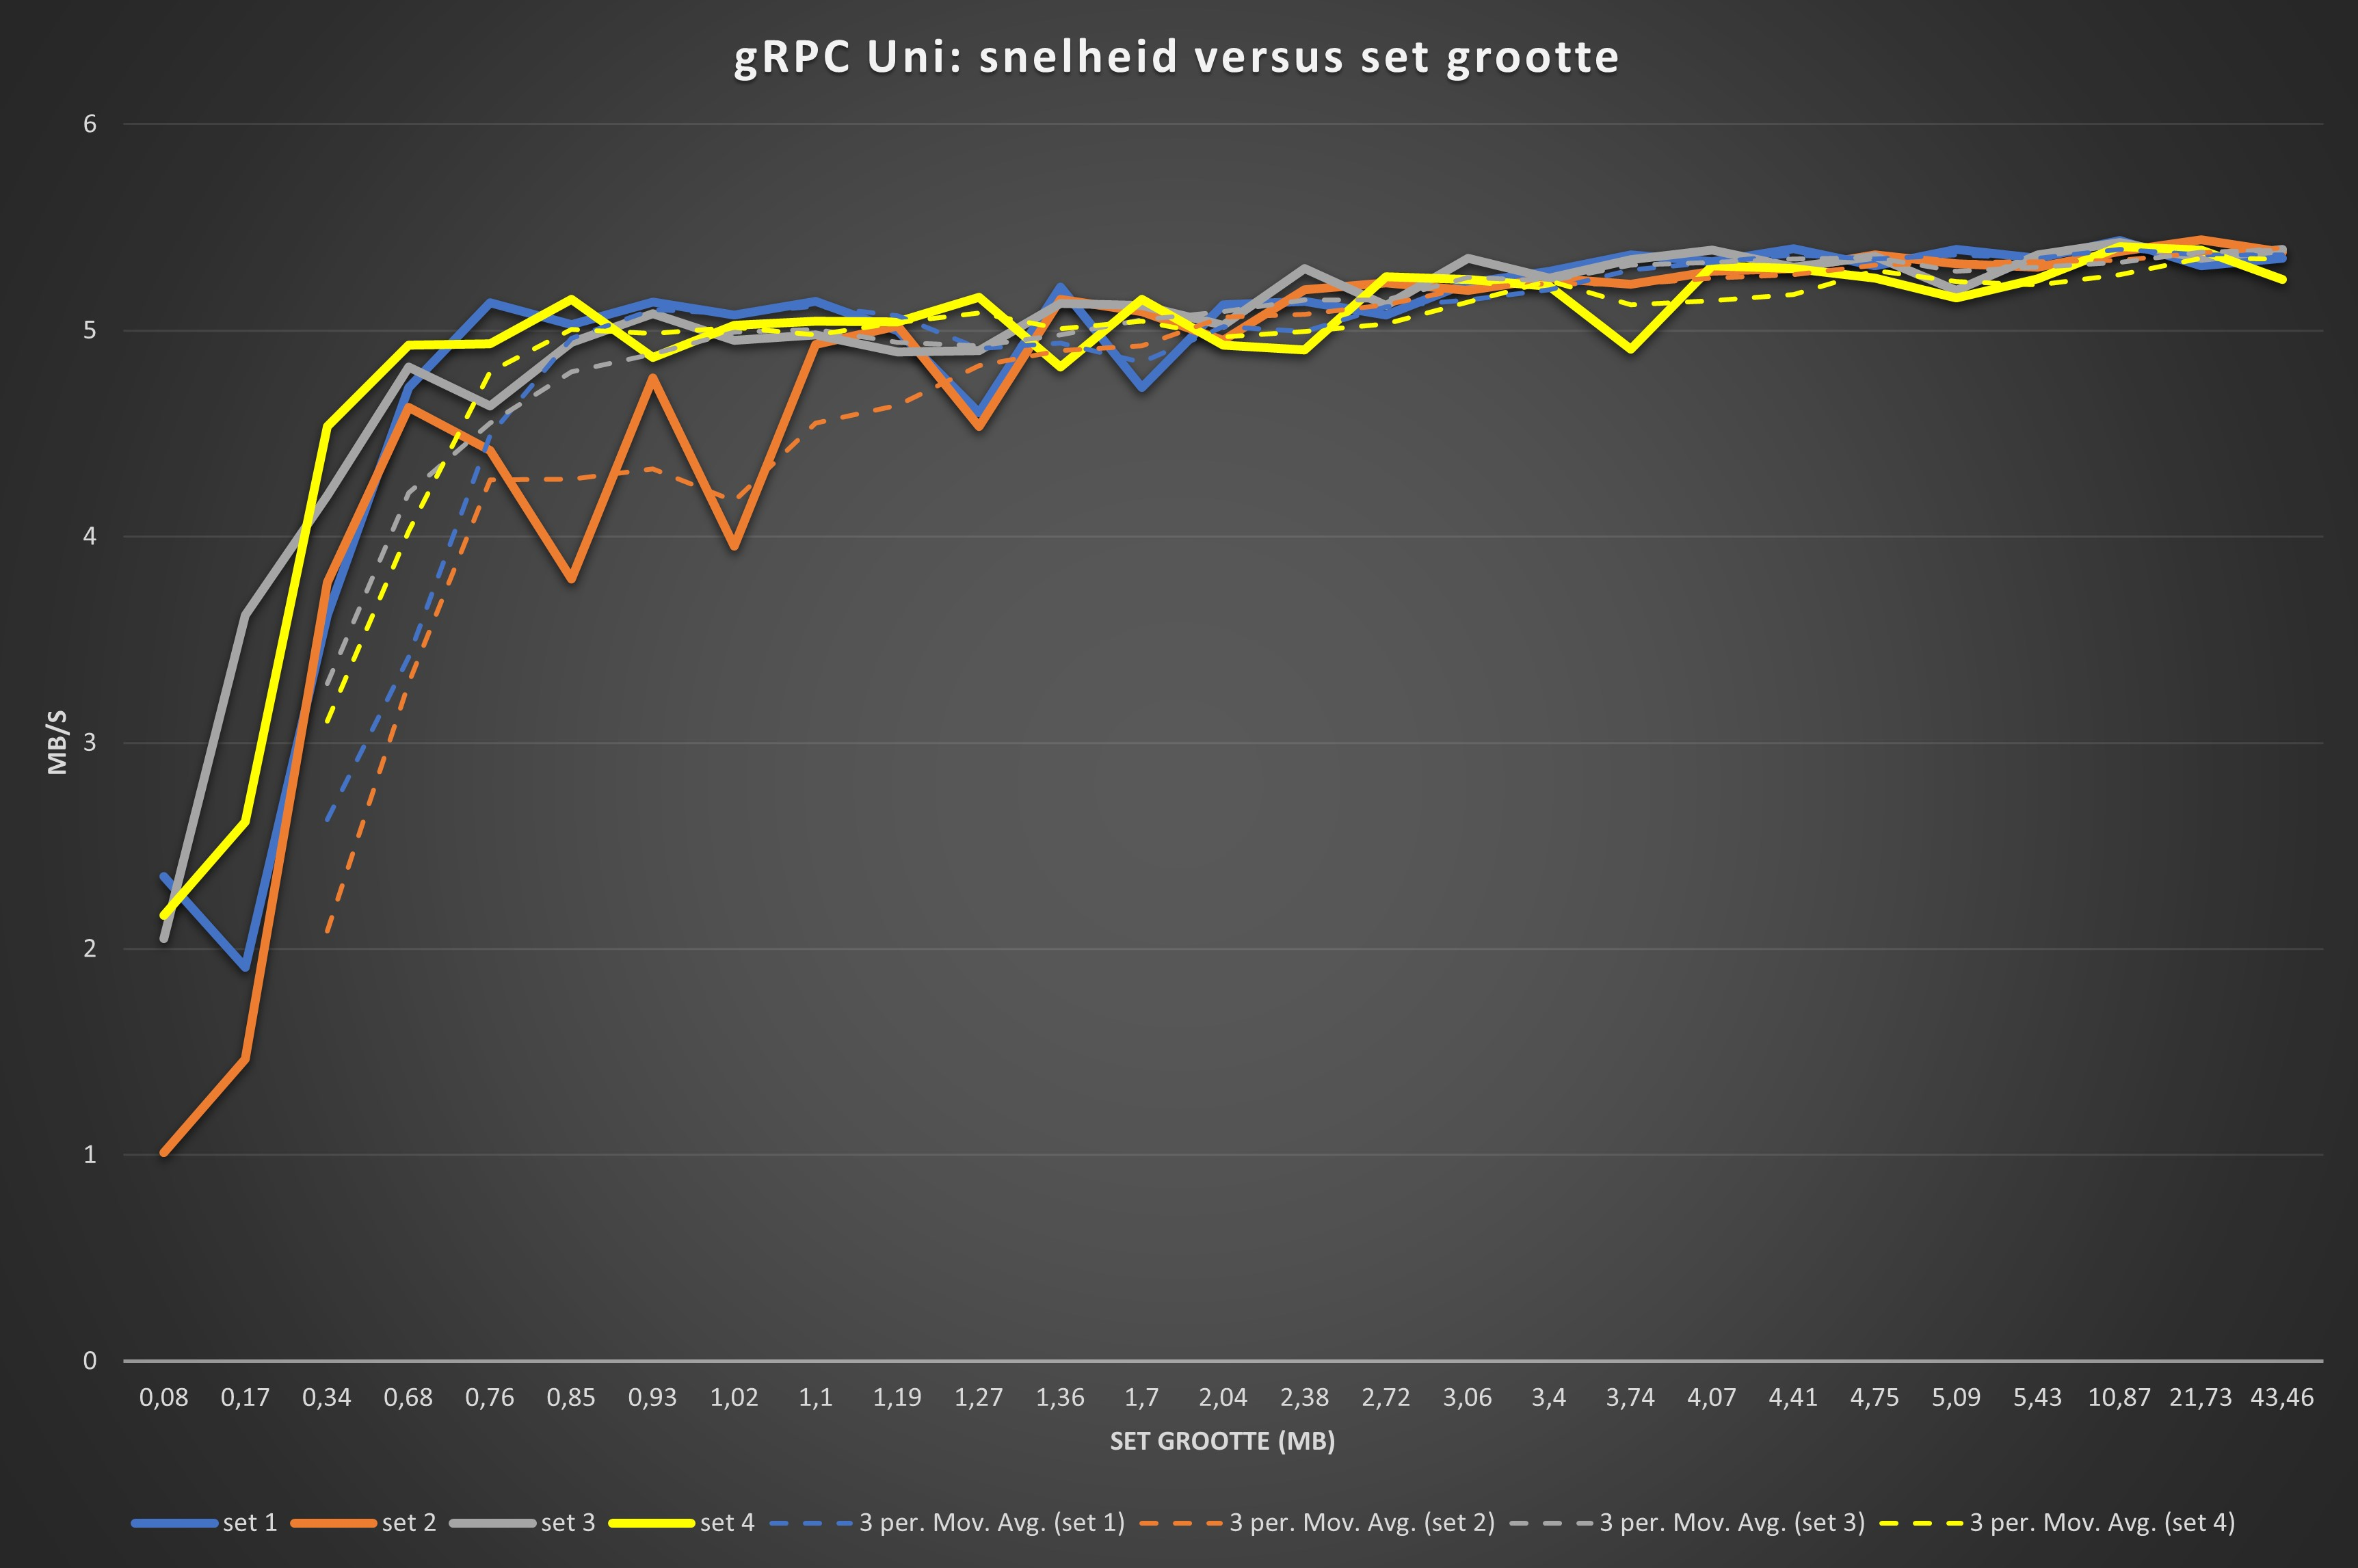
\includegraphics[width=1.0\linewidth]{gRPC_Uni_singular}
    \caption{gRPC Uni - enkelvoudige requests: snelheid vs. datasets van vari\"erende grootte}
    \label{fig:gRPCUnienkelvoudig}
\end{figure}

\textbf{gRPC - Multi}\newline
Het gemiddelde van de performantiemeting van de enkelvoudige requests met de gRPC API functie getPeopleStream, welke een object van het type Multi, en daarmee een stream
teruggeeft, zijn terug te vinden in tabel~\ref{tab:gRPCMultienkelvoudig}
Op figuur~\ref{fig:gRPCMultienkelvoudig} wordt de snelheid in MB/sec weergegeven ten opzichte van de grootte van de verzonden dataset voor de vier sets van
calls die uitgevoerd werden, tevens werden trendlijnen voorzien volgens voortschrijdend gemiddelde over 3 metingen.\\

\begin{table}
    \centering
    \begin{tabular}{llll}
        \toprule
        \textbf{gRPC Multi} & \textbf{Gemiddelde over 4 sets} & \textbf{aze} & \textbf{aze} \\
        \midrule
        Items / call & Groote subset (MB) & tijdsverloop (millies) & snelheid (MB/s) \\
        1024 & 0,08 & 41,5 & 1,927710843 \\
        2048 & 0,17 & 56 & 3,035714286 \\
        4096 & 0,34 & 90,25 & 3,767313019 \\
        8192 & 0,68 & 170,25 & 3,994126285 \\
        9216 & 0,76 & 187,25 & 4,058744993 \\
        10240 & 0,85 & 195 & 4,358974359 \\
        11264 & 0,93 & 217,5 & 4,275862069 \\
        12288 & 1,02 & 242,25 & 4,210526316 \\
        13312 & 1,1 & 259 & 4,247104247 \\
        14336 & 1,19 & 273,5 & 4,351005484 \\
        15360 & 1,27 & 294,5 & 4,312393888 \\
        16384 & 1,36 & 303,75 & 4,477366255 \\
        20480 & 1,7 & 383 & 4,438642298 \\
        24576 & 2,04 & 447,5 & 4,558659218 \\
        28672 & 2,38 & 525,75 & 4,526866381 \\
        32768 & 2,72 & 667,25 & 4,076433121 \\
        36864 & 3,06 & 671,25 & 4,558659218 \\
        40960 & 3,4 & 731 & 4,651162791 \\
        45056 & 3,74 & 807,75 & 4,630145466 \\
        49152 & 4,07 & 882,5 & 4,611898017 \\
        53248 & 4,41 & 964,25 & 4,573502722 \\
        57344 & 4,75 & 1042,75 & 4,555262527 \\
        61440 & 5,09 & 1106,75 & 4,599051276 \\
        65536 & 5,43 & 1168,25 & 4,647977744 \\
        131072 & 10,87 & 2356,5 & 4,612773181 \\
        262144 & 21,73 & 4727,5 & 4,596509783 \\
        524288 & 43,46 & 9285,25 & 4,680541719 \\
         &  &  &  \\
        gemiddelde: &  & 4,271663982 & null \\
        max: &  &  & 4,680541719 \\
        min: & 0 & 0 & 1,927710843 \\
        \bottomrule
    \end{tabular}
    \caption{gRPC Multi - enkelvoudige requests: snelheid vs. datasets van vari\"erende grootte (gemiddelde over 4 sets)}
    \label{tab:gRPCMultienkelvoudig}
\end{table}

\begin{figure}[ht]
    \centering
    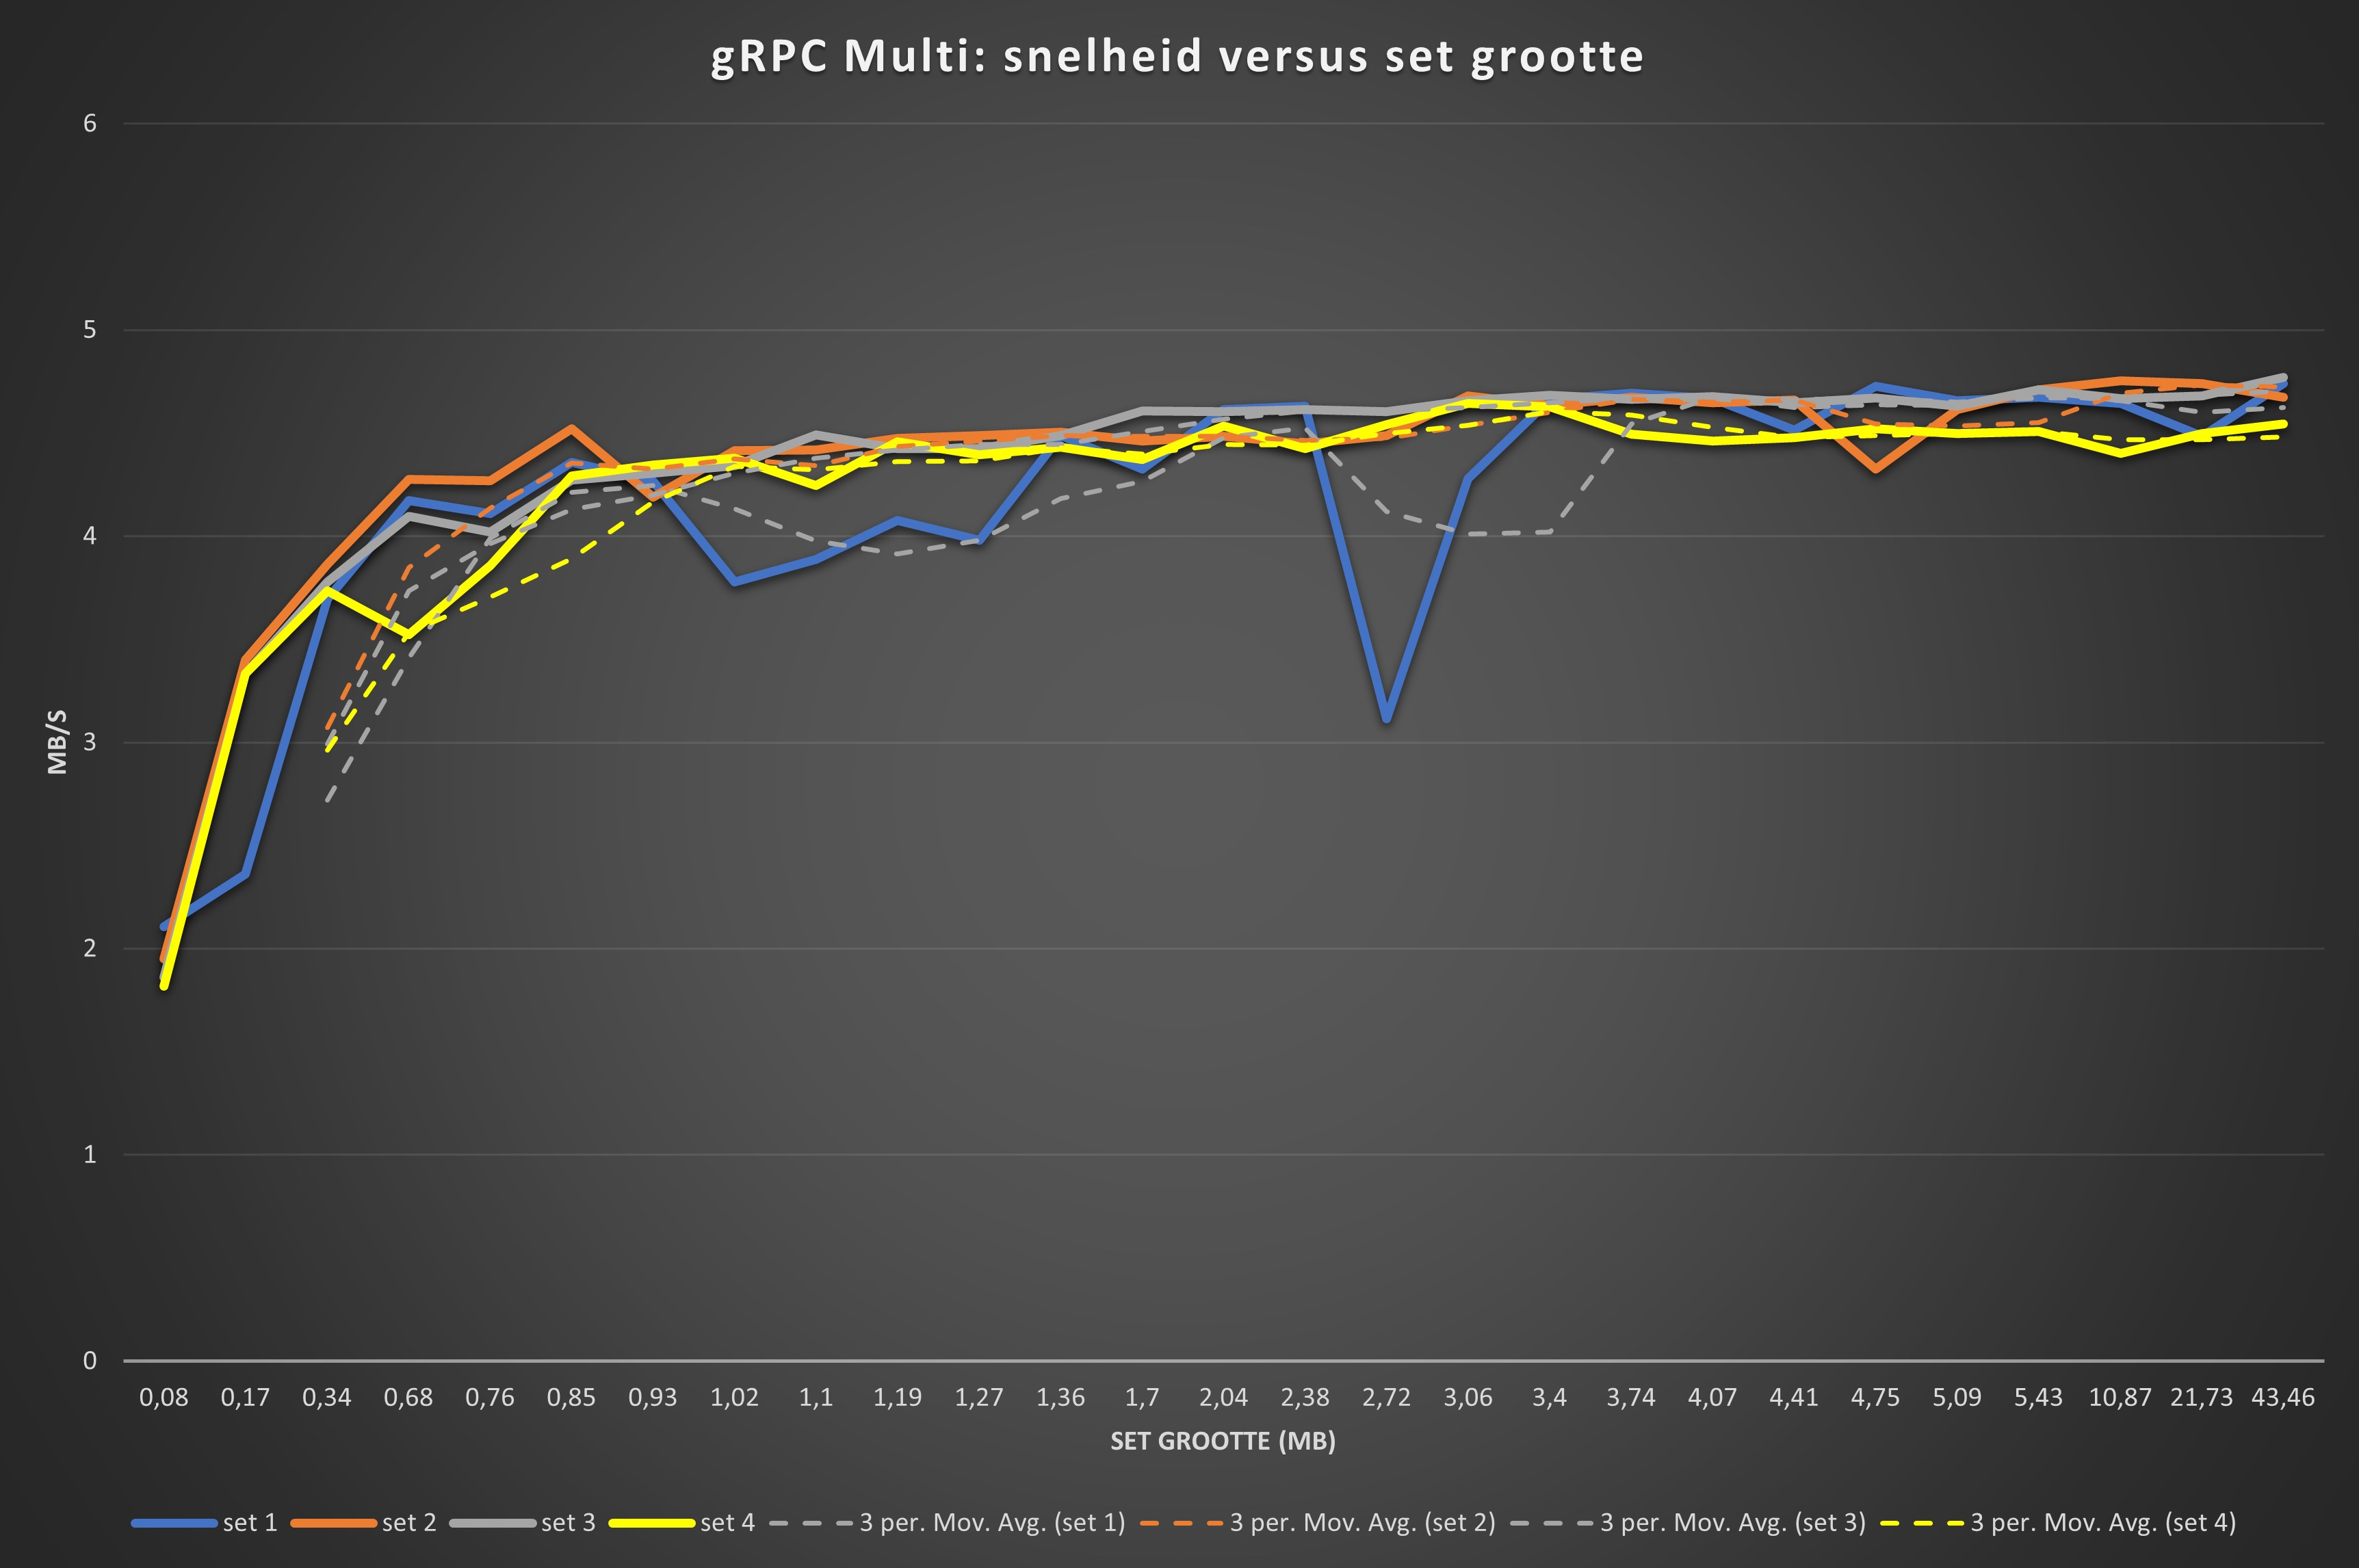
\includegraphics[width=1.0\linewidth]{gRPC_Multi_singular}
    \caption{gRPC Multi - enkelvoudige requests: snelheid vs. datasets van vari\"erende grootte}
    \label{fig:gRPCMultienkelvoudig}
\end{figure}

Tot slot worden de gemiddelde waarden, over de vier sets van calls, voor de vier verschillende types van call samen in een grafiek geplaatst
welke wordt weergegeven in figuur~\ref{fig:RESTRESTcompressiegRPCUnigRPCMulti} alsook worden de gemiddelde tijdsduur per dataset per type call
als percentage weergegeven t.o.v. het tijdsverloop van de meest performante gemiddelde waarde in tabel~\ref{tab:REST_RESTcompressie_gRPCUni_gRPCMultipercentage}\\
\begin{figure}[ht]
    \centering
    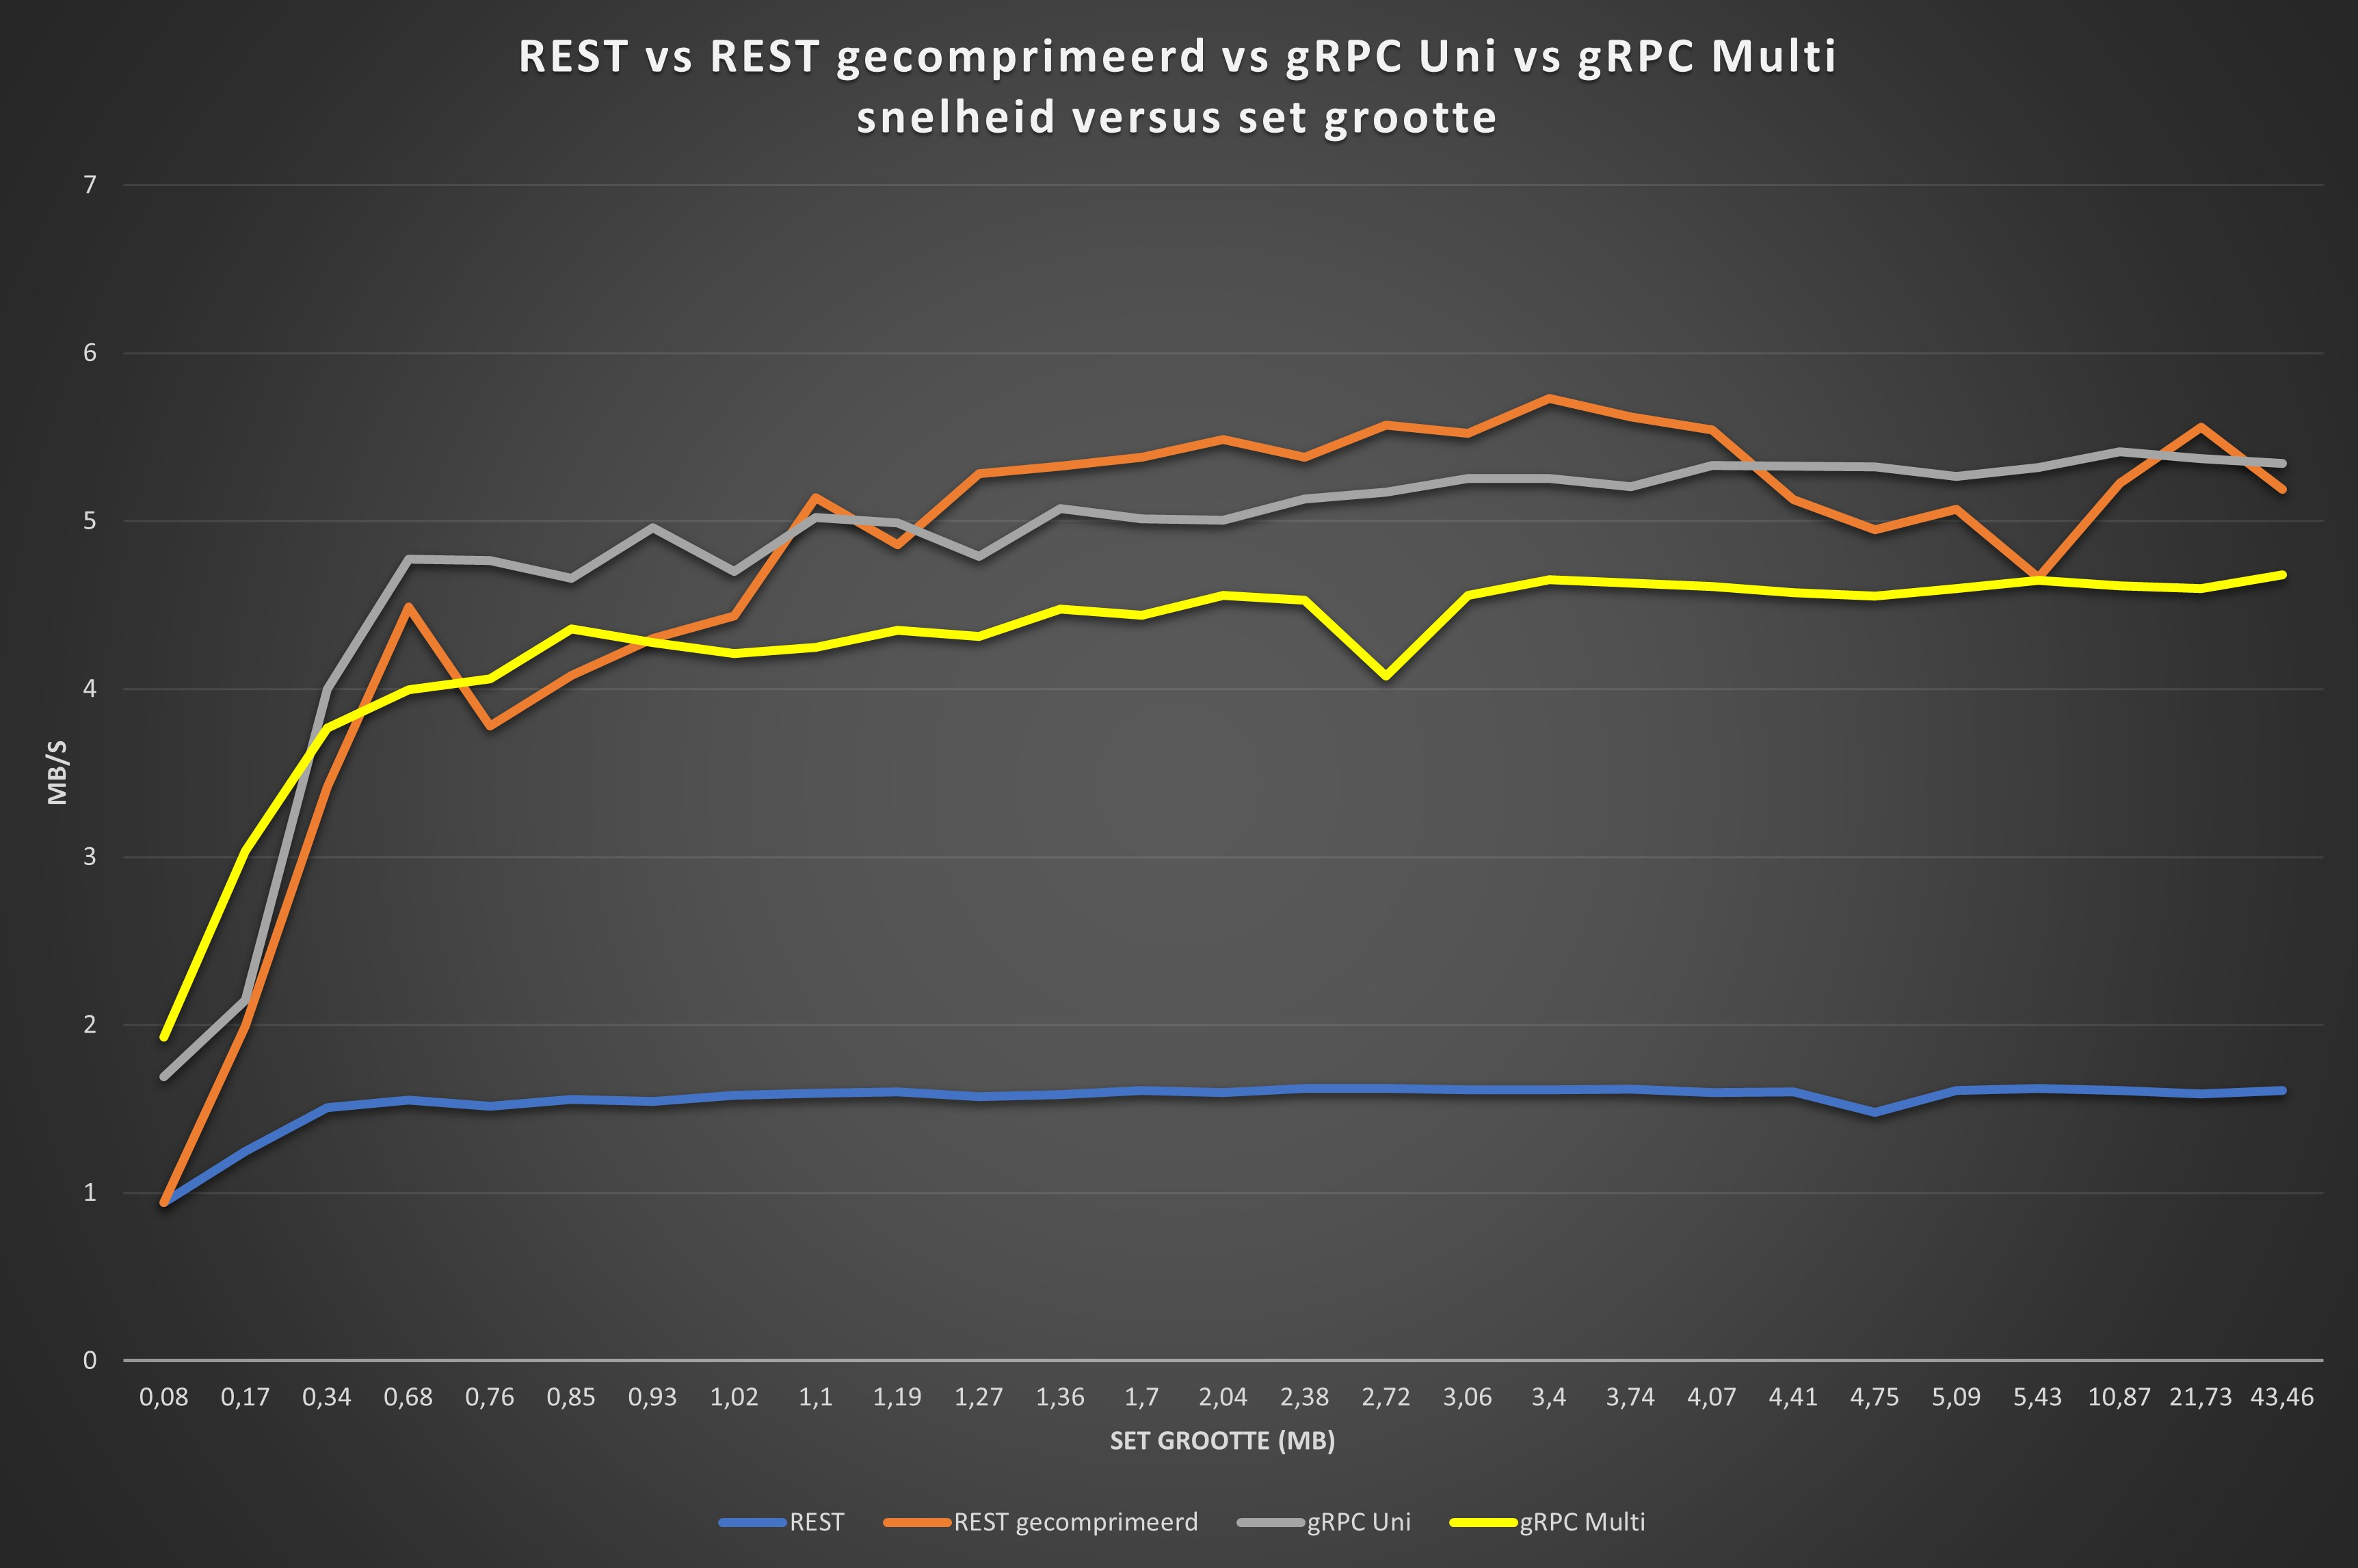
\includegraphics[width=1.0\linewidth]{REST_vs_REST_compressed_vs_gRPC_Uni_vs_gRPC_Multi_singular}
    \caption{REST vs REST met compressie vs gRPC Uni vs gRPC Multi - enkelvoudige requests: snelheid vs. datasets van vari\"erende grootte}
    \label{fig:RESTRESTcompressiegRPCUnigRPCMulti}
\end{figure}

\begin{table}
    \centering
    \begin{tabular}{lllll}
        \toprule
         & \textbf{REST} & \textbf{REST gecomprimeerd} & \textbf{gRPC Uni} & \textbf{gRPC Multi} \\
        \midrule
        Grootte set (MB) &  &  & \\
        0,08 & 204,22\% & 204,22\% & 113,86\% & \textbf{100,00}\% \\
        0,17 & 243,30\% & 152,23\% & 141,52\% & \textbf{100,00}\% \\
        0,34 & 265,59\% & 117,06\% & \textbf{100,00}\% & 106,18\% \\
        0,68 & 307,72\% & 106,32\% & \textbf{100,00}\% & 119,47\% \\
        0,76 & 314,42\% & 126,02\% & \textbf{100,00}\% & 117,40\% \\
        0,85 & 299,32\% & 114,11\% & \textbf{100,00}\% & 106,85\% \\
        0,93 & 321,47\% & 115,33\% & \textbf{100,00}\% & 116,00\% \\
        1,02 & 297,00\% & 105,99\% & \textbf{100,00}\% & 111,64\% \\
        1,1 & 322,78\% & \textbf{100,00}\% & 102,34\% & 121,03\% \\
        1,19 & 311,22\% & 102,73\% & \textbf{100,00}\% & 114,68\% \\
        1,27 & 335,65\% & \textbf{100,00}\% & 110,29\% & 122,45\% \\
        1,36 & 335,95\% & \textbf{100,00}\% & 105,00\% & 119,00\% \\
        1,7 & 334,49\% & \textbf{100,00}\% & 107,28\% & 121,20\% \\
        2,04 & 343,64\% & \textbf{100,00}\% & 109,62\% & 120,38\% \\
        2,38 & 331,92\% & \textbf{100,00}\% & 104,80\% & 118,81\% \\
        2,72 & 343,37\% & \textbf{100,00}\% & 107,73\% & 136,66\% \\
        3,06 & 341,88\% & \textbf{100,00}\% & 105,10\% & 121,16\% \\
        3,4 & 354,74\% & \textbf{100,00}\% & 109,10\% & 123,22\% \\
        3,74 & 347,20\% & \textbf{100,00}\% & 108,04\% & 121,42\% \\
        4,07 & 346,82\% & \textbf{100,00}\% & 103,98\% & 120,19\% \\
        4,41 & 332,55\% & 103,89\% & \textbf{100,00}\% & 116,46\% \\
        4,75 & 359,60\% & 107,62\% & \textbf{100,00}\% & 116,87\% \\
        5,09 & 327,44\% & 103,80\% & \textbf{100,00}\% & 114,48\% \\
        5,43 & 327,86\% & 114,03\% & \textbf{100,00}\% & 114,42\% \\
        10,87 & 336,67\% & 103,59\% & \textbf{100,00}\% & 117,37\% \\
        21,73 & 350,21\% & \textbf{100,00}\% & 103,46\% & 120,94\% \\
        43,46 & 332,13\% & 102,93\% & \textbf{100,00}\% & 114,13\% \\
        \bottomrule
    \end{tabular}
    \caption{Percentage tijdsverloop t.o.v. de performantste meting voor de dataset}
    \label{tab:REST_RESTcompressie_gRPCUni_gRPCMultipercentage}
\end{table}


\paragraph{Meervoudige requests}

De verschillende API's halen hier 4.194.304 items op, via meervoudige calls, welke samen een grootte hebben van 347,68 MB. De grootte van de dataset van de individuele calls
is een variabele.

\textbf{REST - geen compressie}\newline
De resultaten van de performantiemetingen van de meervoudige requests met vari\"erende batch grootte voor REST zonder compressie zijn terug te vinden in tabel~\ref{tab:RESTmeervoudig}.

\begin{table}
    \centering
    \begin{tabular}{lrlll}
        \toprule
        \textbf{REST} & \textbf{\# calls} & \textbf{MB/call} & \textbf{tijdsverloop (s)} & \textbf{snelheid (MB/s)} \\
        \midrule
        4096 x 0,08 & 4096 & 0,08 & 301,757 & 1,152 \\
        2048 x 0,17 & 2048 & 0,17 & 241,451 & 1,440 \\
        1024 x 0,34 & 1024 & 0,34 & 227,211 & 1,530 \\
        512 x 0,68 & 512 & 0,68 & 223,206 & 1,558 \\
        456 x 0,76 & 456 & 0,76 & 220,633 & 1,576 \\
        410 x 0,85 & 410 & 0,85 & 221,524 & 1,569 \\
        373 x 0,93 & 373 & 0,93 & 221,459 & 1,570 \\
        342 x 1,02 & 342 & 1,02 & 220,63 & 1,576 \\
        316 x 1,1 & 316 & 1,1 & 220,668 & 1,576 \\
        293 x 1,19 & 293 & 1,19 & 222,813 & 1,560 \\
        274 x 1,27 & 274 & 1,27 & 220,196 & 1,579 \\
        256 x 1,36 & 256 & 1,36 & 218,817 & 1,589 \\
        205 x 1,7 & 205 & 1,7 & 218,281 & 1,593 \\
        171 x 2,04 & 171 & 2,04 & 219,916 & 1,581 \\
        147 x 2,38 & 147 & 2,38 & 222,171 & 1,565 \\
        128 x 2,72 & 128 & 2,72 & 219,802 & 1,582 \\
        114 x 3,06 & 114 & 3,06 & 257,891 & 1,348 \\
        103 x 3,4 & 103 & 3,4 & 277,943 & 1,251 \\
        94 x 3,74 & 94 & 3,74 & 236,711 & 1,469 \\
        86 x 4,07 & 86 & 4,07 & 225,356 & 1,543 \\
        79 x 4,41 & 79 & 4,41 & 216,78 & 1,604 \\
        74 x 4,75 & 74 & 4,75 & 225,515 & 1,542 \\
        69 x 5,09 & 69 & 5,09 & 220,718 & 1,575 \\
        64 x 5,43 & 64 & 5,43 & 232,757 & 1,494 \\
        32 x 10,87 & 32 & 10,87 & 215,222 & 1,615 \\
        \textbf{16 x 21,73} & \textbf{16} & \textbf{21,73} & \textbf{214,471} & \textbf{1,621} \\
        8 x 43,46 & 8 & 43,46 & 217,293 & 1,600 \\
        \bottomrule
    \end{tabular}
    \caption{REST - meervoudig}
    \label{tab:RESTmeervoudig}
\end{table}

\textbf{REST - geen compressie}\newline
De resultaten van de performantiemetingen van de meervoudige requests met vari\"erende batch grootte voor REST zonder compressie zijn terug te vinden in tabel~\ref{tab:RESTcompressiemeervoudig}.

\begin{table}
    \centering
    \begin{tabular}{lrlll}
        \toprule
        \textbf{REST gecomprimeerd} & \textbf{\# calls} & \textbf{MB/call} & \textbf{tijdsverloop (s)} & \textbf{snelheid (MB/s)} \\
        \midrule
        4096 x 0,08 & 4096 & 0,08 & 167,581 & 2,075 \\
        2048 x 0,17 & 2048 & 0,17 & 105,843 & 3,285 \\
        1024 x 0,34 & 1024 & 0,34 & 77,894 & 4,464 \\
        512 x 0,68 & 512 & 0,68 & 71,712 & 4,848 \\
        456 x 0,76 & 456 & 0,76 & 70,355 & 4,942 \\
        410 x 0,85 & 410 & 0,85 & 71,543 & 4,860 \\
        373 x 0,93 & 373 & 0,93 & 68,853 & 5,050 \\
        342 x 1,02 & 342 & 1,02 & 66,463 & 5,231 \\
        316 x 1,1 & 316 & 1,1 & 66,269 & 5,246 \\
        293 x 1,19 & 293 & 1,19 & 65,376 & 5,318 \\
        274 x 1,27 & 274 & 1,27 & 66,452 & 5,232 \\
        256 x 1,36 & 256 & 1,36 & 75,157 & 4,626 \\
        205 x 1,7 & 205 & 1,7 & 62,569 & 5,557 \\
        171 x 2,04 & 171 & 2,04 & 64,519 & 5,389 \\
        147 x 2,38 & 147 & 2,38 & 61,571 & 5,647 \\
        128 x 2,72 & 128 & 2,72 & 60,401 & 5,756 \\
        114 x 3,06 & 114 & 3,06 & 60,366 & 5,760 \\
        103 x 3,4 & 103 & 3,4 & 60,897 & 5,709 \\
        94 x 3,74 & 94 & 3,74 & 59,975 & 5,797 \\
        86 x 4,07 & 86 & 4,07 & 61,437 & 5,659 \\
        79 x 4,41 & 79 & 4,41 & 59,937 & 5,801 \\
        74 x 4,75 & 74 & 4,75 & 61,758 & 5,630 \\
        69 x 5,09 & 69 & 5,09 & 60,036 & 5,791 \\
        \textbf{64 x 5,43} & \textbf{64} & \textbf{5,43} & \textbf{59,063} & \textbf{5,887} \\
        32 x 10,87 & 32 & 10,87 & 59,711 & 5,823 \\
        16 x 21,73 & 16 & 21,73 & 60,034 & 5,791 \\
        8 x 43,46 & 8 & 43,46 & 59,82 & 5,812 \\
        \bottomrule
    \end{tabular}
    \caption{REST gecomprimeerd - meervoudig}
    \label{tab:RESTcompressiemeervoudig}
\end{table}

\textbf{gRPC Uni}\newline
De resultaten van de performantiemetingen van de meervoudige requests met vari\"erende batch grootte voor gRPC API functie getPeople, welke een object van het type Uni teruggeeft, zijn
terug te vinden in tabel~\ref{tab:gRPCUnimeervoudig}.

\begin{table}
    \centering
    \begin{tabular}{lrlll}
        \toprule
        \textbf{gRPC Uni} & \textbf{\# calls} & \textbf{MB/call} & \textbf{tijdsverloop (s)} & \textbf{snelheid (MB/s)} \\
        \midrule
        4096 x 0,08 & 4096 & 0,08 & 168,927 & 2,058 \\
        2048 x 0,17 & 2048 & 0,17 & 99,498 & 3,494 \\
        1024 x 0,34 & 1024 & 0,34 & 78,463 & 4,431 \\
        512 x 0,68 & 512 & 0,68 & 73,046 & 4,760 \\
        456 x 0,76 & 456 & 0,76 & 70,555 & 4,928 \\
        410 x 0,85 & 410 & 0,85 & 72,944 & 4,766 \\
        373 x 0,93 & 373 & 0,93 & 69,503 & 5,002 \\
        342 x 1,02 & 342 & 1,02 & 69,755 & 4,984 \\
        316 x 1,1 & 316 & 1,1 & 69,913 & 4,973 \\
        293 x 1,19 & 293 & 1,19 & 69,08 & 5,033 \\
        274 x 1,27 & 274 & 1,27 & 68,361 & 5,086 \\
        256 x 1,36 & 256 & 1,36 & 68,588 & 5,069 \\
        205 x 1,7 & 205 & 1,7 & 68,454 & 5,079 \\
        171 x 2,04 & 171 & 2,04 & 68,704 & 5,061 \\
        147 x 2,38 & 147 & 2,38 & 66,767 & 5,207 \\
        128 x 2,72 & 128 & 2,72 & 66,338 & 5,241 \\
        114 x 3,06 & 114 & 3,06 & 66,598 & 5,221 \\
        103 x 3,4 & 103 & 3,4 & 66,256 & 5,248 \\
        94 x 3,74 & 94 & 3,74 & 66,749 & 5,209 \\
        86 x 4,07 & 86 & 4,07 & 66,131 & 5,257 \\
        79 x 4,41 & 79 & 4,41 & 68,542 & 5,073 \\
        74 x 4,75 & 74 & 4,75 & 66,461 & 5,231 \\
        69 x 5,09 & 69 & 5,09 & 66,155 & 5,256 \\
        64 x 5,43 & 64 & 5,43 & 65,984 & 5,269 \\
        32 x 10,87 & 32 & 10,87 & 70,275 & 4,947 \\
        16 x 21,73 & 16 & 21,73 & 65,573 & 5,302 \\
        \textbf{8 x 43,46} & \textbf{8} & \textbf{43,46} & \textbf{65,201} & \textbf{5,332} \\
        \bottomrule
    \end{tabular}
    \caption{gRPC Uni - meervoudig}
    \label{tab:gRPCUnimeervoudig}
\end{table}

\textbf{gRPC Multi}\newline
Tot slot is het resultaat van de performantiemeting van de enkelvoudige stream requests voor gRPC API functie getPeopleStream,
welke een object van het type Multi, en dus een stream teruggeeft, dat de hele 4.194.304 items werden ontvangen door de client 73.964 millies of 73,964 seconden
na het aanroepen van de gRPC functie.\\

\begin{table}
    \centering
    \begin{tabular}{lllll}
        \toprule
        \textbf{} & \textbf{REST} & \textbf{REST gecomprimeerd} & \textbf{gRPC Uni} & \textbf{gRPC Multi} \\
        \midrule
        tijdverloop (s) & 214,471 & 59,063 & 65,201 & 73,964 \\
        percentage & 363,12\% & \textbf{100,00\%} & 110,39\% & 125,23\% \\
        \bottomrule
    \end{tabular}
    \caption{Percentage tijdsverloop t.o.v. de performantste meting voor de het versturen van }
    \label{tab:REST_RESTgecomprimeerd_gRPCUni_gRPCmultimeervoudig}
\end{table}


\textbf{Logs performantiemetingen}\newline
Alle logs die geleid hebben tot de resultaten die in dit onderzoek zijn voorgesteld, alsook de excel bestanden waarin de resultaten zijn verwerkt en de grafieken gecre\"eerd,
zijn terug te vinden op de reeds vermelde publieke GIT repository op GITHUB via https://github.com/thiersnicolas/gRPC\_vs\_REST in volgende folders.\newline
Voor alle documenten met betrekking tot het REST API:\newline
application\_client/infrastructure/dataproviders/dataproviders-rest/src/test/resources/final\newline
Voor alle documenten met betrekking tot de gRPC API.\newline
application\_client/infrastructure/dataproviders/dataproviders-grpc/src/test/resources/final\\

\section{Conclusie}

\paragraph{Enkelvoudige requests}
De resultaten van de performantiemetingen tijdens de enkelvoudige requests bevestigen deels wat de stand van zaken reed deed vermoeden nl. een gRPC API is out of the box
meer performant dan een standaard REST API. De cijfers die hier naar boven komen in tabel\ref{tab:REST_RESTcompressie_gRPCUni_gRPCMultipercentage} m.b.t.
het hier ge\"{\i}mplementeerde REST API met JSON zonder compressie en het gRPC API met Unary methode wijzen, bij heel kleine datasets van maximum enkele honderd bytes, erop dat gRPC
daarbij ongeveer dubbel zo snel is. Bij iets grotere datasets tot de limiet getest in dit onderzoek, welke 43,46MB bedraagt, stijgt dit verschil tot 3,5 keer.
De grafiek in figuur~\ref{fig:RESTRESTcompressiegRPCUnigRPCMulti} toont ook heel duidelijk aan dat het standaard REST API met JSON het minst performant is.\\
In een gRPC API wordt de data reeds standaard gecomprimeerd. Bij een REST API is dit echter ook een optie, zo werd reeds in de stand van zaken naar voor gebracht. Wanneer er
in tabel\ref{tab:REST_RESTcompressie_gRPCUni_gRPCMultipercentage} naar de verhouding tussen REST gecomprimeerd en gRPC Uni gekeken wordt valt op dat het REST API met gebruik van compressie
zelfs vaak het meeste performantste is. Het is de moeite waard om nogmaals te melden dat gzip gesupporteerd wordt door nagenoeg alle moderne browsers terwijl dit juist een pijnpunt is voor gRPC.\\

\paragraph{Meervoudige requests}
De eerdere resultaten bekomen bij de testen van de enkelvoudige requests zijn gelijkaardig aan diegene die hier kunnen vastgesteld worden. Weer is het standaard
REST API zonder compressie het minst performante. Het ziet er zelfs naar uit dat de verhouding iets groter geworden is. Weer opmerkelijk komt het REST API
met compressie echter naar boven als meest performante.\\

Gezien het mogelijk is om een REST API ongeveer even performant te maken als een gRPC API lijkt het bij het overwegen van beide API's voor een nieuwe applicatie
belangrijk rekening te houden met het gegeven dat gRPC niet ondersteund wordt door browsers. Daar komt bij dat REST zeer wijdverspreid en veelgebruikt is, zoals gebleken
uit de stand van zaken, en, ondanks dat gRPC in opmars is, het verschil tussen beide technologi\"en op dat vlak groot is. Voor beide API's is het noodzakelijk om
de client te informeren over de werking, het zgn. contract. Voor REST zijn er op vandaag verschillende mogelijkheden om het API contract bloot te stellen aan clients.
Voor gRPC komt de moeilijkheid van het delen van het .proto bestand daarentegen aan bod. Tot slot het reeds meermaals herhaalde punt nl. dat browsers REST ondersteunen, en zelfs
een REST API dat gebruik maakt van compressie, terwijl dit voor gRPC niet het geval is.

\paragraph{Toekomstig onderzoek}
Om dit onderzoek zo compleet mogelijk te maken werd het gRPC API voorzien van een functie dat een stream doorgeeft.
De belangstelling hiervoor is snel gedaald zodra bleek dat deze, zelfs bij grotere datasets die niet in één request konden verzonden worden.
De implementatie was echt eenvoudig zonder dat er bij de server applicatie bepaalde processen vooraf gingen aan het kunnen versturen van de dataset.
Ook was er geen achterliggen verwerkingsproces bij de client na ontvangst van de data.
Het lijkt een interessant onderzoeksonderwerp om na te gaan voor welke scenario's een dergelijk streaming API wel de kroon spant en,
gezien de grotere technische moeilijkheid, hoe de implementatie dan praktisch zou verlopen.
